Suppose we have generated a test input that has caused invalid observations of
the SUT.  The generated counterexample consists of (1) {\em signals} that are
essential to triggering violations, and (2) {\em noises} that do not contribute
to revealing such violations.  We need to shrink the counterexample by removing
its noises and keeping its signals.

For interactive testing, the test input is a sequence of request messages.  An
intuitive way of shrinking is to remove some requests from the original sequence
and rerun the test.  However, rerunning an interesting request might produce
trivial results, due to inter-execution nondeterminism discussed in
\autoref{sec:inter-execution}.

To prevent turning signals into noises when rerunning the test, I shrink the
heurestics instead of shrinking the generated test input.
\autoref{sec:shrink-architecture} introduces the architecture for interactive
shrinking, then \autoref{sec:shrink-ir} explains the language design beneath
that addresses inter-execution nondeterminism.

\subsection{Architecture}
\label{sec:shrink-architecture}

I propose a generic framework for generating and shrinking interactive tests.
The key idea is to introduce an abstract representation for test inputs that
embed trace-based heuristics.  When shrinking the counterexample, the test
harness picks a substructure of the abstract representation, and computes the
corresponding test input using the new runtime trace.

For example, when generating a timestamp, instead of producing concrete value
{\it e.g.} ``\httpdate\today~\currenttime~GMT'', the generator returns an
abstract representation that says ``use the timestamp observed in the last
response''.  When rerunning the test, the timestamp is computed from the new
trace {\it e.g.} ``\httpdate\DayAfter~\currenttime~GMT''.

\begin{figure}
  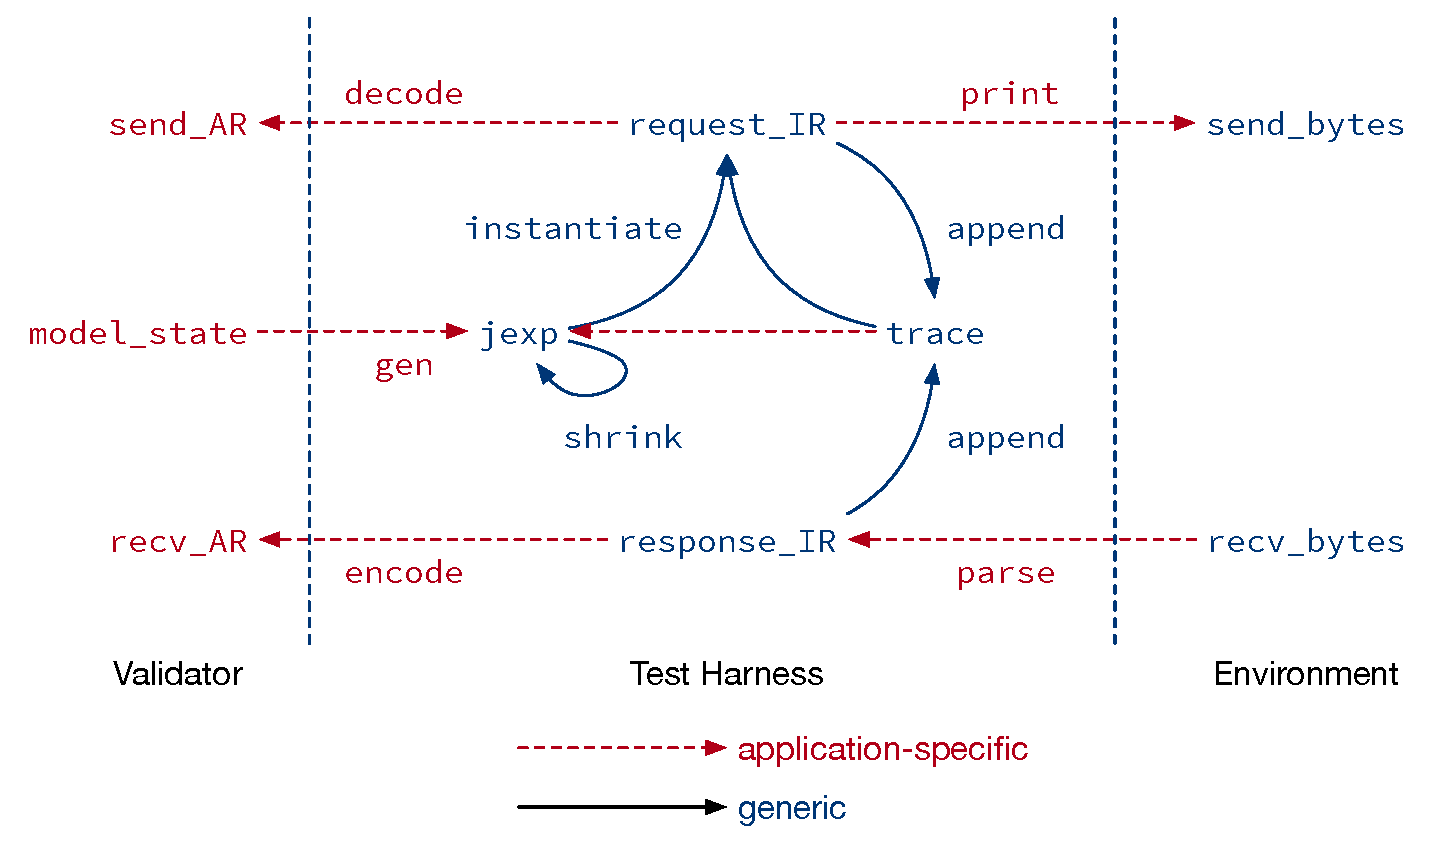
\includegraphics[width=.8\textwidth]{figures/shrink}
  \caption{Test harness architecture.}
  \label{fig:shrink}
\end{figure}

The test generation and shrinking framework is shown in \autoref{fig:shrink}.
It refines the test harness box in \autoref{fig:overview}, and involves four
languages, from right to left:
\begin{enumerate}
  \item Byte representation, in which the tester interacts with the environment.
    This can be network packets, file contents, or other serialized data
    produced and observed by the tester.
  \item Intermediate representation (IR), a generic language that abstracts the
    byte representation as structured data.  The test harness {\em parses} byte
    observations and records its trace in terms of the IR, which allows
    representing trace-based heuristics as a generic language {\it i.e.}
    J-expressions.
  \item J-expression (Jexp), a symbolic abstraction of the IR.  The IR
    corresponds to concrete inputs and outputs, whereas Jexp defines a
    computation from trace to IR.  The generator provides test inputs in terms
    of Jexps; The test harness {\em instantiates} the generated Jexps into
    request IR, and {\em prints} them into byte representation.

    When shrinking test inputs, the test harness shrinks the sequence of Jexps.
    The shrunk Jexps are then instantiated by the new trace during runtime.

    The intermediate representation and J-expression will be further explained
    in \autoref{sec:shrink-ir}.
  \item Application representation (AR), including the request (\ilc Q),
    response (\ilc A), and state (\ilc S) types used for specifying the
    protocol.  Specification writers can choose the type interface at their
    convenience, provided the request and response types are embeddable into the
    IR.
\end{enumerate}

The testing framework implements protocol-independent mechanisms like recording
the trace and shrinking counterexamples, based on the generic IR and Jexp
languages.  It can be used for testing various protocols, provided
application-specific translations from IR to AR and between IR and bytes.  The
test developer needs to tune the generator that produces Jexps, encoding their
domain knowledge as state-based and trace-based heuristics.

\subsection{Abstract representation languages}
\label{sec:shrink-ir}
I choose JSON as the IR in this framework, which allows syntax trees to be
arbitrarily wide and deep, and provides sufficient expressiveness for encoding
message data types in general.

\begin{figure}
\[\begin{array}{r@{\;}l}
\mathsf{JSON^T}\triangleq&\mathsf T\mid\{\mathsf{object^T}\}\mid[\mathsf{array^T}]\mid\mathsf{string}\mid\Int\mid\Bool\mid\mathsf{null}\\
\mathsf{object^T}\triangleq&\nil\mid\mathsf{"string": JSON^T,object^T}\\
\mathsf{array^T}\triangleq&\nil\mid\mathsf{JSON^T,array^T}\\
\mathsf{IR}\triangleq&\mathsf{JSON^{IR}}\\
\mathsf{Jexp}\triangleq&\mathsf{JSON^{\Jref{\mathit{label}}{\Jpath}{\mathit{function}}}}\\
&\text{where }\mathit{label}\in\Nat,\mathit{function}\in\mathsf{IR}\to\mathsf{IR}\\
\Jpath\triangleq&\This\mid\Jpath\Number\mathit{index}\mid\Jpath\At\mathit{field}\\
&\text{where }\mathit{index}\in\Nat,\mathit{field}\in\mathsf{string}
\end{array}\]
\caption{Intermediate representation and J-expression.}
\label{fig:ir-jexp}
\end{figure}

The J-expression is an extension of JSON that can encode trace-based heuristics.
As shown in \autoref{fig:ir-jexp}, a Jexp may include syntax
$(label.\Jpath.function)$ that represents trace-based heuristics, specified as:
\begin{enumerate}
\item $label$
\item $\Jpath$
\item $function$
\end{enumerate}
